\chapter{Eigenvalue solver}
\label{ch:eiv}

Here we give some information on the usage of the eigenvalue solver, implemented
in GKW, as well as some technical details. 
Further information can be found in the presentation of R. Buchholz on the GKW webpages under Talks.

As the system size of the linear gyrokinetic equation is too big for a direct numerical solution, projection
methods are used.
For a brief introduction to projection methods, see the {\sc slepc} manual \cite{SLE12} and references therein.


\section{Usage}
\label{sec:eivusage}
First, GKW must be compiled with {\sc slepc/petsc}, see \ref{subsubsec:slepc}
for details.

The easiest way to create an input file for the eigenvalue solver is the following:
First, set up an input file which uses explicit time
integration.
As second step then replace \name{METHOD = 'EXP'} with \name{METHOD='EIV'}
and  set \name{METH=1}. It is recommended to set a low value \name{NAVERAGE} like \name{NAVERAGE=1}.
Setting \name{METH=2} or \name{NAVERAGE$\gg$1} works too, but the run is then usually slower.

The third and final step is to set the parameters for the eigenvalue solver
itself. This is done in the namelist \name{eiv_integration},
an example of which is given below.
One has to select the portion of the spectrum to be sought with the parameter \name{which_eigenvalues}. Available options are listed in the sample input file.
In addition, you can choose between two methods for extracting eigenvalues,
\name{type_extraction = 'harmonic'}, and \name{type_extraction = 'ritz'}.
Note that with \name{type_extraction = 'harmonic'} the target values \name{growthrate} and \name{freq}) are always used. 

Unfortunately it is difficult to recommend optimal settings in advance,
or even settings which will guarantee to find physically interesting eigenmodes of the system.

One rule seems to be valid in general:
If you use harmonic extraction and search for the mode with largest
eigenvalue, you should keep the target frequency \name{freq=0.0}.  
If you don't find an eigenvalue, increase the target \name{growthrate}, 
while if you just find stable high frequency eigenmodes, decrease it.

To share some experiences, fig. \ref{fig:eivharmonicgrowth}--\ref{fig:eivtargetsa} 
show scans for two sets of parameters.
\begin{figure}[htp!]
  \begin{center}
    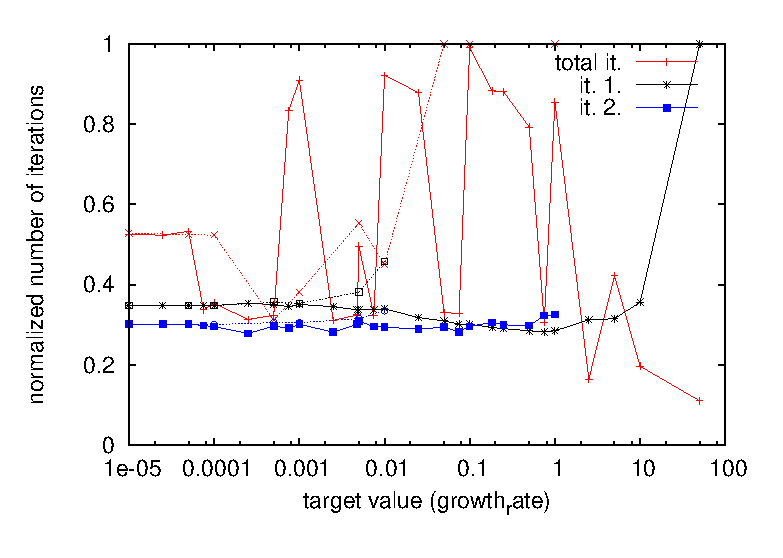
\includegraphics[width=0.8\textwidth]{HarmonicGrowth}
    \caption{\label{fig:eivharmonicgrowth} Scan over growth rate with
    frequency set to zero. Dashed lines depict negative values of
    \name{growthrate}. Normalization is done with the maximum number of
    iterations for the first/second eigenvalue/total number of iterations,
    respectively.}
  \end{center}
\end{figure}
\begin{figure}[htp!]
  \begin{center}
    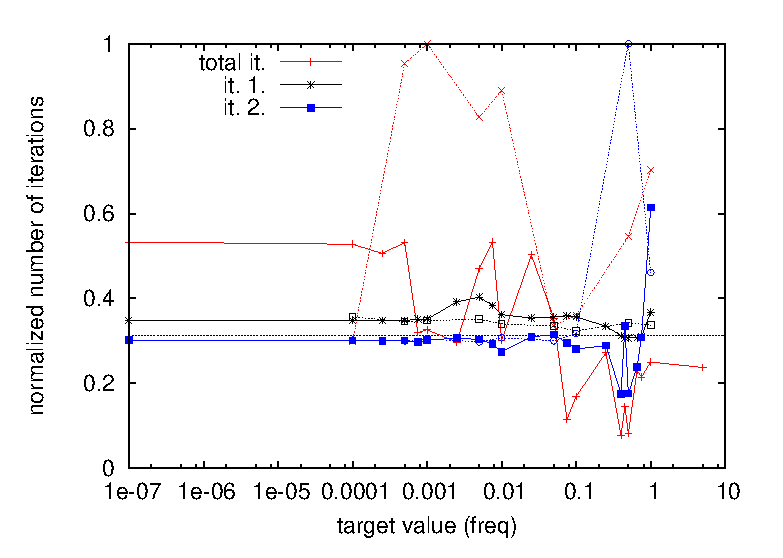
\includegraphics[width=0.8\textwidth]{HarmonicFreq}
    \caption{\label{fig:eivharmonicfreq} Scan over frequency with growth rate
      set to zero. Dashed lines depict negative values of \name{freq}. The
      point at $10^{-7}$ actually had zero frequency. Normalization is as for
      fig. \ref{fig:eivharmonicgrowth}. The dashed-dotted line depicts the
      minimum value for the total iterations of fig. \ref{fig:eivharmonicgrowth}
      (only counting points where both unstable eigenmodes are found).}
  \end{center}
\end{figure}
\begin{figure}[htp!]
  \begin{center}
    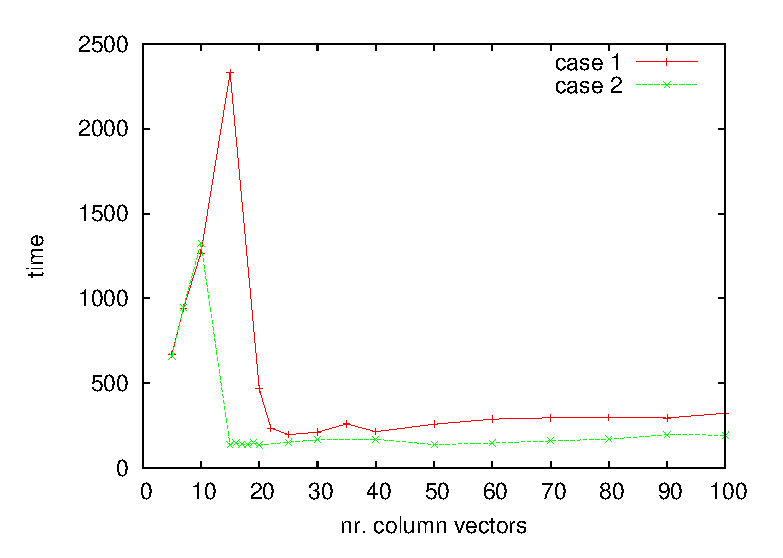
\includegraphics[width=0.8\textwidth]{HarmonicNcv}
    \caption{\label{fig:eivharmonicncv} Scan over size of subspace  (\name{nr\_column\_vec}), for one
    point of each of the other two scans. First case: \name{growthrate = 0.0},
    freq = 0.45, searching for 5 eigenpairs (default value: 20). Second case: growthrate = 2.50E-3,
    freq = 0.0, searching for 2 eigenpairs (default value: 17).}
  \end{center}
\end{figure}

The input parameters for fig. \ref{fig:eivtargets1}--\ref{fig:eivtargetsa} are
based on the \File{STD_linear_ITG} and \File{simple_TEM} input files found in
\File{doc/input}, with $R/L_{T_i} = 6$, which is near the ITG-TEM transition.
Two unstable eigenmodes are therefore expected.
Scans were made over the target \name{growthrate} and \name{freq} for the harmonic extraction.
The fixed parameters for the eigenvalue solver were
\begin{verbatim}
max_iterations = 30000
tolerance = 1.0e-6
type_solver = 'krylovschur'
type_extraction = 'harmonic'
number_eigenvalues = 3 ! just in case there are more unstable ones than expected
nr_column_vec      = 20
mat_vec_routine    = 1
which_eigenvalues =  1 ! largest magnitude
\end{verbatim}

\begin{figure}[htp!]
  \begin{center}
    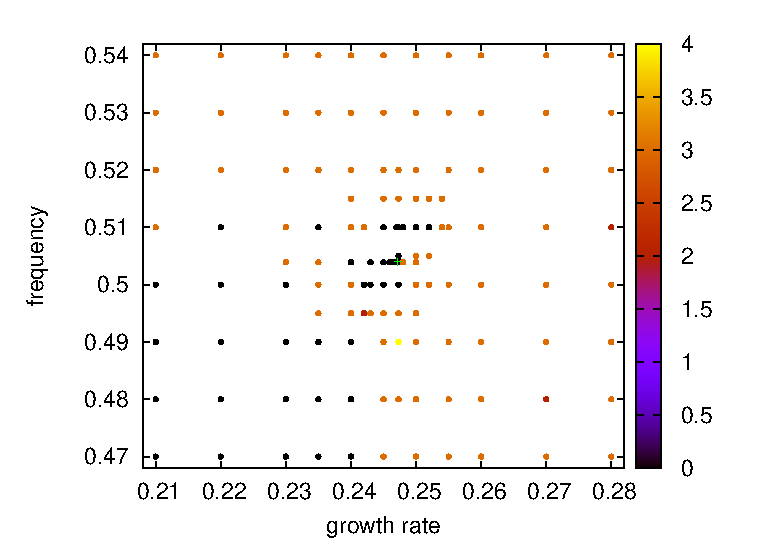
\includegraphics[width=0.8\textwidth]{Targets}
    \caption{\label{fig:eivtargets1} A scan over target values near the ITG,
      searching for eigenvalues with largest magnitude.
      Plus signs refer to actual found eigenvalues, crosses to 'conjugated'
      eigenvalues, stars to the projections on the growth rate axis. Color
      of the dots refers to the number of found eigenvalues. Please note, that
      a value of 1(or more) requires that the fastest growing eigenmode was found and
      a value of 2(or more) requires that both fastest growing eigenmodes where found.
      Harmonic extraction was used.      
}
  \end{center}
\end{figure}
\begin{figure}[htp!]
  \begin{center}
    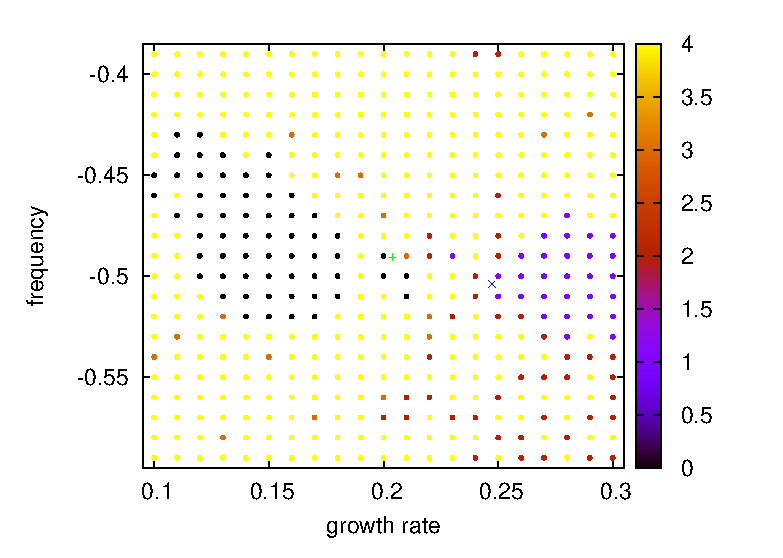
\includegraphics[width=0.8\textwidth]{Targets2}
    \caption{\label{fig:eivtargets2} A scan analogous to \ref{fig:eivtargets1}, 
      but target values are near the TEM eigenvalue.
      For the meaning of the symbols please refer to the caption of fig.
      \ref{fig:eivtargets1}.}
  \end{center}
\end{figure}
\begin{figure}
  \begin{center}[htp!]
    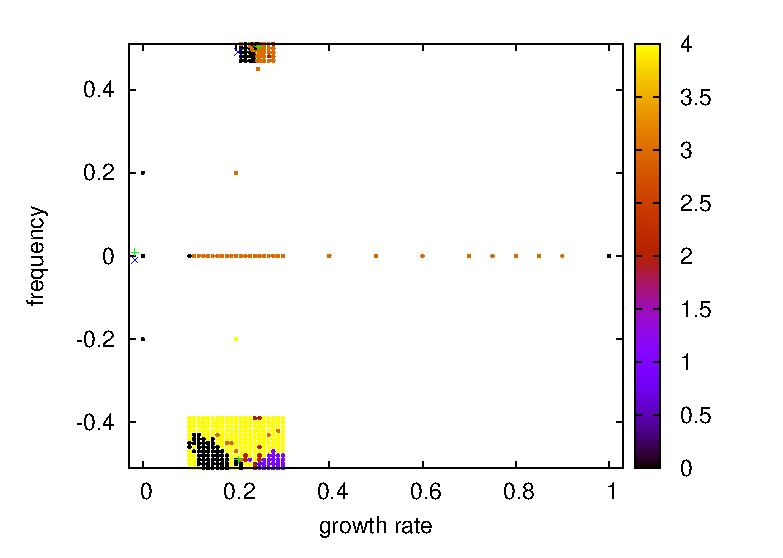
\includegraphics[width=0.8\textwidth]{TargetsA}
    \caption{\label{fig:eivtargetsa} A scan over the target values searching for eigenvalue with largest magnitude, with harmonic extraction.
      Scan along \name{freq = 0}, some of the other two scans can also be
      seen.
      For the meaning of the symbols please refer to the caption of fig.
      \ref{fig:eivtargets1}.}
  \end{center}
\end{figure}

If you just want to find the fastest growing
eigenmode, there is not much variation in the speed a solution is found.
 In the examples here, 900-1000 iterations were
needed (if a mode was found at all). This is different though for the violet points,
 which needed 6000-8000 iterations.
For the second eigenvalue the situation is
quite samilar. It is typically found 100-150 iterations after the first one in
the case of fig. \ref{fig:eivtargets1}, whereas for fig. \ref{fig:eivtargets2}
it is found even quicker. Finding a third (stable) eigenvalue may then take several thousand further iterations.  
Wasting computing time unnecessarily can be avoided by setting a suitable value for max_iterations,
setting \name{max_seconds} or by observing the log and placing a \name{gkw.stop} if desired.\\

Robustness and speed of the solver are very dependent on the initial condition.
We found \name{finit='cosine4'} to be a good choice, but when
doing a parameter scan, it can also be useful to restart with the output of the previous
run.  The batch launcher \scripts{gkwnlin} provides the feature (\name{-restart_chain}) for doing 
this.

The diagnostic output is only written when the solver finishes,
i.e. as soon as the requested number of eigenvalues is found, the
maximum number of iterations is reached, 
or the solver stops due to \name{gkw.stop} or \name{max_seconds}. 
No diagnostic output is produced if the code is killed preliminarly by the queuing system.

The diagnostic output differs from the output obtained with \name{method = 'EXP'}.
The main difference is that eigenmode index takes the place of the time in time-dependent datasets.\\
 For example, the first line in \File{fluxes.dat} will contain
the fluxes computed for the first eigenmode, the second line those for
the second eigenmode, and so on.

You will also notice that instead of a single \File{parallel.dat} or restart file, one for each found eigenmode is produced.

Furthermore, there is an diagnostic output \File{eigenvalues} that contains the growth
rate and frequency determined by {\sc slepc} (first column acts as an index).

If eigenvalues are found, you should check that these belong to a
reasonable, physical mode. If
the eigenvalues computed by the \name{diagnos_growth_freq} diagnostics and the one
determined by slepc (found in \File{eigenvalues.dat}) differ this is a sign
that the result may be unphysical. 
Another possibility to check this is to plot the mode structure.
Note that some of the eigenvalues found could be physical while others
are not. In particular for stable eigenmodes, different parallel decompositions 
 may result in different eigenmodes being found, 

%-----------------------------------------------------------------------------

\section{Technical details}
\label{sec:eivtechdetails}
The eigenvalue solver in {\sc gkw} is mainly a interface for the library
 {\sc slepc} (which relies on {\sc petsc}).

Most parameters of the \name{eiv_integration} namelist are directly passed down to
 {\sc slepc}.

Note that no matrix is given to {\sc slepc}, as the so called matrix-free approach
is used. This means instead of a matrix we define the action of the matrix
on a vector via a function, provided to {\sc slepc}.
%This approach is used as the actual matrix is not available.
Depending on the settings in the input file, either \code{exp_integration} 
(\name{mat_vec_routine = 1}) is used
to determine the result of the matrix vector multiplication or just the subroutine
\code{calculate_rhs} (\name{mat_vec_routine = 2}).

%-----------------------------------------------------------------------------

\subsection{The actual eigenvalue problem}
\label{subsec:eivproblem}
In general an eigenvalue problem is formulated as
\begin{equation}
  A x = \lambda x, \label{eq:eivgen}
\end{equation}
where $A$ is the operator of the problem and $\lambda$ is the (complex)
eigenvalue.
The \code{exp_integration()} routine computes
\begin{equation}
  f_{t+1} = f_{t} + dt A f_{t} + dt B \phi
\end{equation}
\begin{equation}
  0 = C f_{t} + D \phi
\end{equation}
where $A$, $B$, $C$ and $D$ are matrices and the vectors $f$ and $\phi$
represent all the fields that may be present in the simulation.
Note that GKW works with a vector \code{fdisi} = ($f, \phi$).

In principle it is possible to solve the field equation for $\phi$ and insert
it into the evolution equation to get
\begin{equation}
  f_{t+1} = f{t} + dt A f_{t} - dt B D^{-1} C f_{t}.
\end{equation}
The disadvantage of this approach is, that the inversion of the matrix $D$
and the matrix matrix multiplication most probably would destroy the sparsity
structure of the complete operator. 
This would make the determination of the eigenvalues much more expensive.
For this reason the actual matrix of this problem is not explicitly formulated.

%-----------------------------------------------------------------------------

\subsection{Transformation between eigenvalue and growth rate/frequency}
\label{subsec:eivtrafoeivgf}
The transformation between the complex eigenvalue computed by SLEPC and the growth
rate and frequency in terms of GKW can be derived as follows.
In comparison to the eigenvalue problem formulated in \eqref{eq:eivgen}, 
the eigenvalue problem in GKW is
\begin{equation}
  l f =  (1 + dt N)^n f
\end{equation}
where $N$ stands for the effective matrix of evolution and field equation and $n$ is \code{naverage}.
Identifying $M$ and $(1 + dt N)^n$ results in
\begin{equation}
  \lambda = (1 + dt N) = l
\end{equation}
\begin{equation}
  \ln \lambda = n \ln l
\end{equation}

\begin{equation}
  \frac{\ln \lambda}{n dt} = \frac{\ln l}{n dt}
\end{equation}
The right hand side of these equation is the same relation as between the
change in the norm and the growth rate in the code. We take this as reason to
propose this as general transformation between the eigenvalue found by slepc and
the growth rate and frequency as commonly used in GKW.

\newcommand{\pder}[2]{\frac{\partial#1}{\partial#2}}
The transformation for the tolerance $a$ is
\begin{align}
	a_{gkw} & = & \sqrt{\left( \pder{\lambda_{gkw}}{\lambda_{slepc}} |\lambda_{slepc}|a_{slepc}\right)^2} \\
	& = & \sqrt{\left( \pder{(\log(\lambda_{slepc})/(n_{average} \Delta t))}{\lambda_{slepc}} |\lambda_{slepc}|a_{slepc}\right)^2} \\
	& = & \sqrt{\left( \frac{1}{n_{average} \Delta t} a_{slepc}\right)^2} \\
	& = & \frac{a_{slepc}}{n_{average} \Delta t}
\end{align}


%-----------------------------------------------------------------------------

\section{\label{sec:eivfaq}FAQ}

\paragraph{What is a good starting point for the parameters?}

For the Ritz extraction
to find the two most unstable modes you could try
\begin{verbatim}
&CONTROL
 fac_dtim_est=0.5, naverage= 1, method= 'EIV', meth= 1,
 read_file = .true., irun = 2   ! to restart from previous dominant mode
 ! using gkwnlin -restart_chain
 max_seconds = 10000 ! adjust the runtime
 /
&EIV_INTEGRATION
 max_iterations = 90000
 tolerance=1.0e-4
 number_eigenvalues=2
 type_extraction = 'ritz'
 which_eigenvalues=3 ! search for most unstable modes
 /
\end{verbatim}
It seems that the timestep must not be larger than that required for explicit time integration
but that setting a very small timestep makes the convergence take longer.
Setting the tolerance too small can also cause convergence to take longer, and can even prevent finding
the correct modes.

For the harmonic extraction, you can try the following.
\begin{verbatim}
 &CONTROL
 fac_dtim_est=0.5,
 naverage= 1,
 method= 'EIV',
 meth= 1,
 max_seconds = 10000 ! adjust the runtime
 /
 &EIV_INTEGRATION
 max_iterations = 90000
 tolerance = 1.0e-4
 type_extraction = 'harmonic'
 number_eigenvalues = 2
 nr_column_vec      = 20
 mat_vec_routine    = 1
 which_eigenvalues  = 8 ! look for eigenvalues near the target growthrate
 growthrate = 0.5000 
 freq = 0.0000
 /
 &SPCGENERAL
 finit="cosine4"
 /
 \end{verbatim}
If you increase \code{number_eigenvalues} you may also have to increase
\code{nr_column_vec}.

\paragraph{Does \code{nr_column_vec = 0} (letting 'PETSC_DECIDE') work?}

From the scan done over the size of the subspace (see fig. \ref{fig:eivharmonicncv}
we would expect, that it should work well for at least \code{number_eigenvalues = 1-2}.
For bigger values it might be not optimal.\\
Experience shows that even for \code{number_eigenvalues = 15} eigenvalues 
were found.

\paragraph{I try to compile in single precision/default real but
eiv_integration.F90 fails./Testcases fail after I fix the errors.}
You probably have to configure {\sc pets}c/{\sc slep}c
 \code{--with-precision=single} (as of 3.6.2). It has not been checked if the
code then actually works, though.
Just fixing the bugs that prevent compiling is not enough as there will still
be a type mismatch between the vectors used by {\sc slep}c and the arrays
used by gkw.

\paragraph{How Do I find the number of iterations at which an eigenmode was found?}
You can find this information in the screen output as soon as
converged modes are found. You may stop the run at any time
by creating a \name{gkw.stop} file.

% \paragraph{Is there a way to output eigenmodes as they are found, instead
% of waiting until the end or the maximum number of iterations ?}

% \paragraph{Doesn't the optimal nr_colum_vec increase with the problem size ?}

% related to auctex mode and latex-preview-mode in Emacs:
%%% Local Variables:
%%% mode: latex
%%% TeX-master: "doc"
%%% End:
